\subsubsection{XCS}
\index{XCS}
ZCS has many positive features, especially its simplicity and the benefits derived from its cooperative fitness sharing, but there are some notable drawbacks, primarily that it usually will not evolve a complete mapping of the environmental states and allowable actions to the possible rewards, often quickly selects local optima, and breeds across niches, as noted in \cite{Wilson1995XCS}.
These drawbacks led Wilson to heavily modify ZCS into what is called XCS \cite{Wilson1995XCS}.
In XCS, several of the deficiencies in ZCS are addressed.
The basic structure of XCS is graphically illustrated in Figure~\ref{fig:xcs}.

In ZCS, the GA is run on the entire population, a \emph{panmictic} approach \cite[p.~155]{EibenSmith}.
This is ineffective for most problems, so in XCS the GA was run only in the current match set at the time step that the GA is run in the initial version of XCS, and only in the current action set at the time step that the GA is run in the later variants of XCS.
We run the GA on the current action set in this work.
This allows for a more accurate rule set to be evolved, since each niche is best viewed as its own sub-problem.

In ZCS, a rule is allowed to survive by the GA on the basis of its payoff.
This is problematic,
since it biases against rules early in a chain of events that are eventually profitable,
and because rules that may be the most appropriate for an event might have a relatively low payoff.
This caused ZCS to often fail to create a complete mapping and fail to evolve accurate generalizations.
This is remedied in XCS by creating a fitness measure for the rules, separate from the predicted payoff, used by the GA.

\begin{figure}
\begin{center}
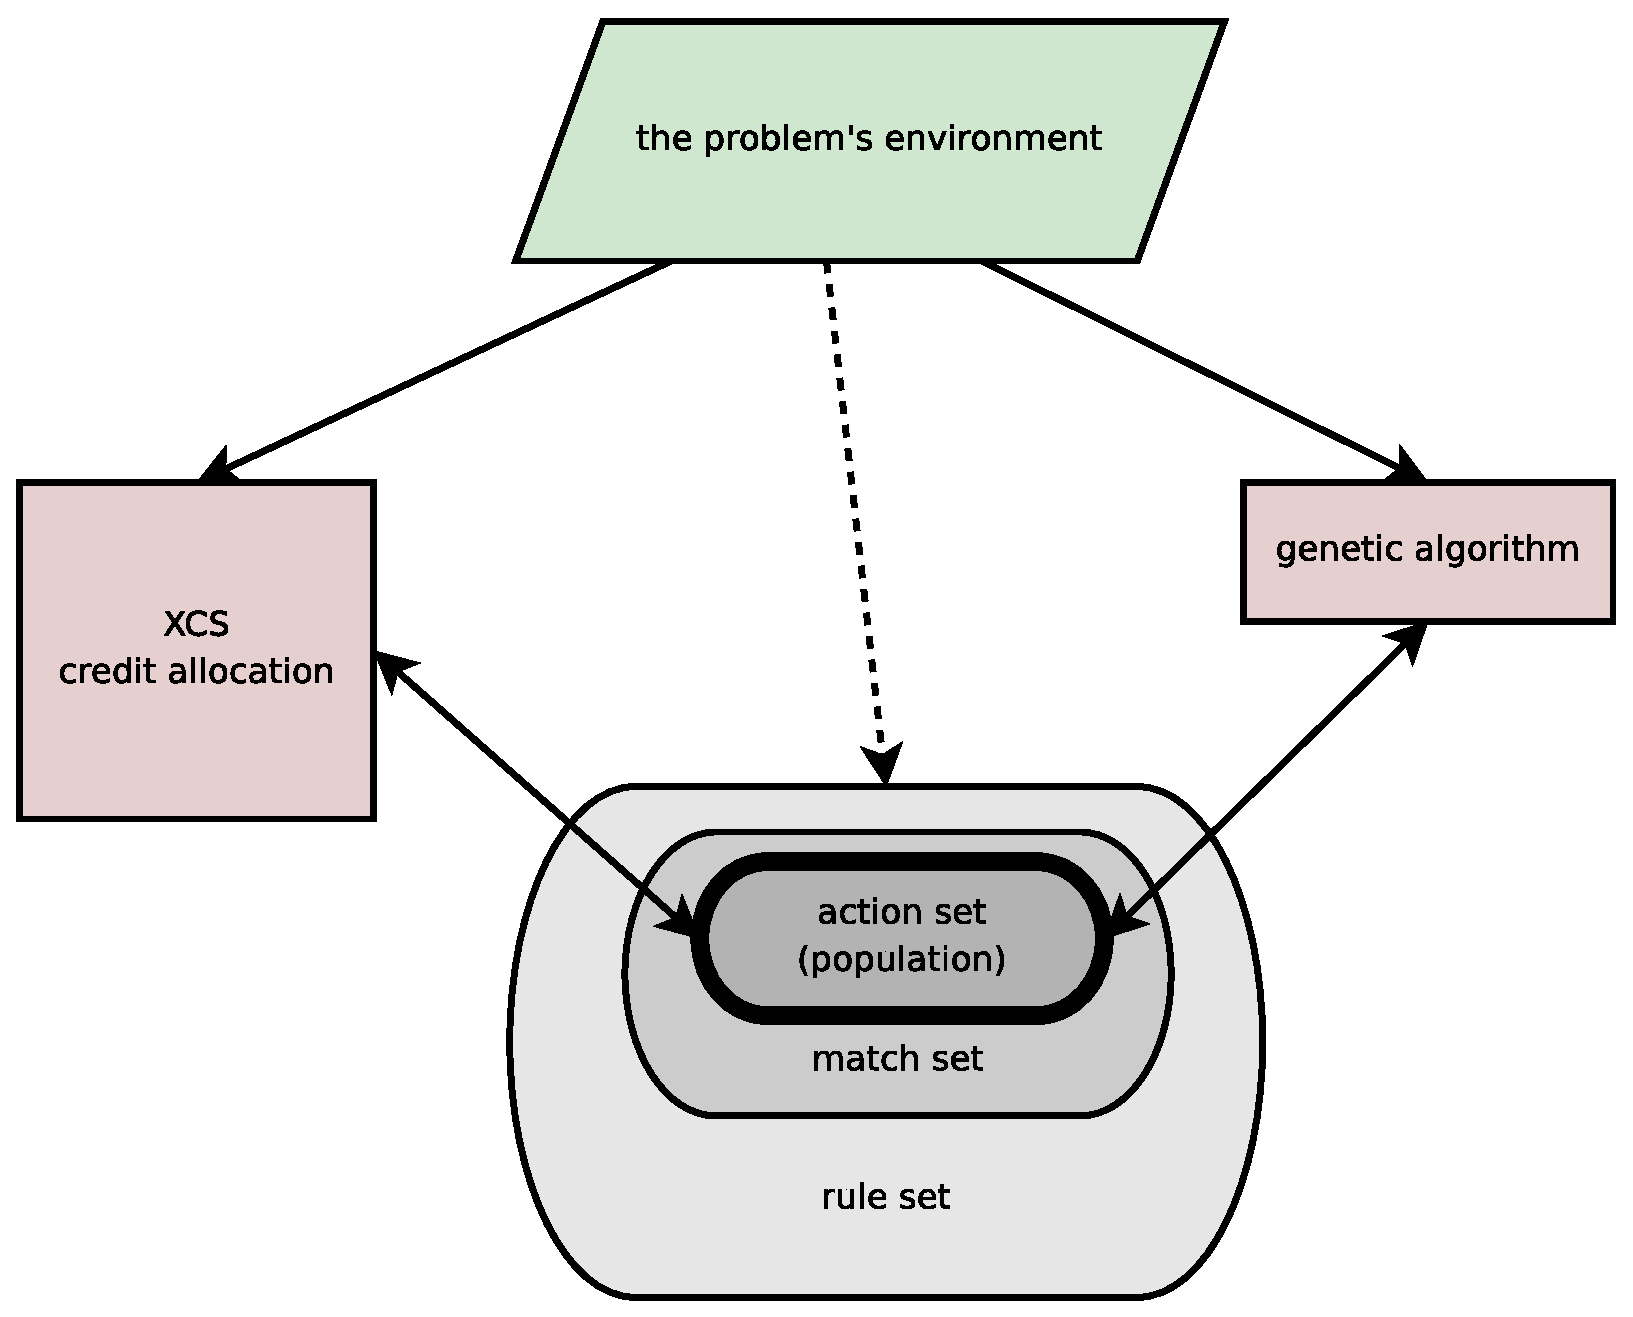
\includegraphics[width=4in]{xcs-basic-diagram.eps}
\caption{XCS's basic structure}
\label{fig:xcs}
\end{center}
\end{figure}

Each rule $r$ is now of the  more complex form
\begin{equation}
r = (c, a, p, \epsilon, F, exp, ts, as, n),
\end{equation}
where:
\begin{itemize}
\item
$c$ is the condition matched by the rule $r$, comprised of elements from some alphabet such as $\{0, 1, \#\}$,
where \# is the matching symbol, matching both 0 and 1.
\item
$a$ is the action that the rule $r$ recommends.
\item
$p$ is the predicted payoff.
\item
$\epsilon$ is an estimate of the prediction error.
\item
$F$ is the fitness used by the GA.
It is vital that the fitness used by the GA is a measure of the \emph{accuracy} of the rule,
and not a measure of the \emph{magnitude} of the rule, where the magnitude of a rule is how active that rule is in relation to the rest of the rules in the rule set, since a rule with greater magnitude but lower accuracy can be a detriment to the system.
For example, a rule that always matched every situation (all \#'s in the condition) but only accurately predicted 51\% of the situations would have high magnitude but low accuracy.
\item
$exp$ is the experience of the rule,
a count of the number of times since this classifier's creation that it has belonged to the action set.
\item
$ts$ is a time stamp of the last occurrence of a call to the GA in an action set that this classifier was a part of, as the generational number.
\item
$as$ is an estimate of the average action set size this classifier has belonged to.
\item
$n$ is the numerosity of this macro-classifier.
This is how many traditional micro-classifiers this macro-classifier represents.
Groups of entirely identical normal classifiers (the micro-classifiers) are subsumed into macro-classifiers instead of being allowed to exist separately within the rule set; this serves solely as a computational time-saver.
Therefore the only difference between a normal classifier (a micro-classifier) and a macro-classifier is the presence of the numerosity, which is a count of how many micro-classifiers that specific macro-classifier represents.
\end{itemize}
